\section{Data Quality} \label{sec:res_DataQuality}

\subsection{Raw data accuracy and resolution}

Initial hardware implementation show the accuracy of data from the eye tracker in question. Figure \ref{fig:res_FirstHeatMapTest} show the first heat map generated. This heat map was generated from a few minutes of reading the first page of a general scientific paper full screen on a 1920x1200 monitor. As we can see, the eye tracker has an accuracy which allows for clear distinctions of paragraphs and lines.

\begin{figure}[h]
    \centering
    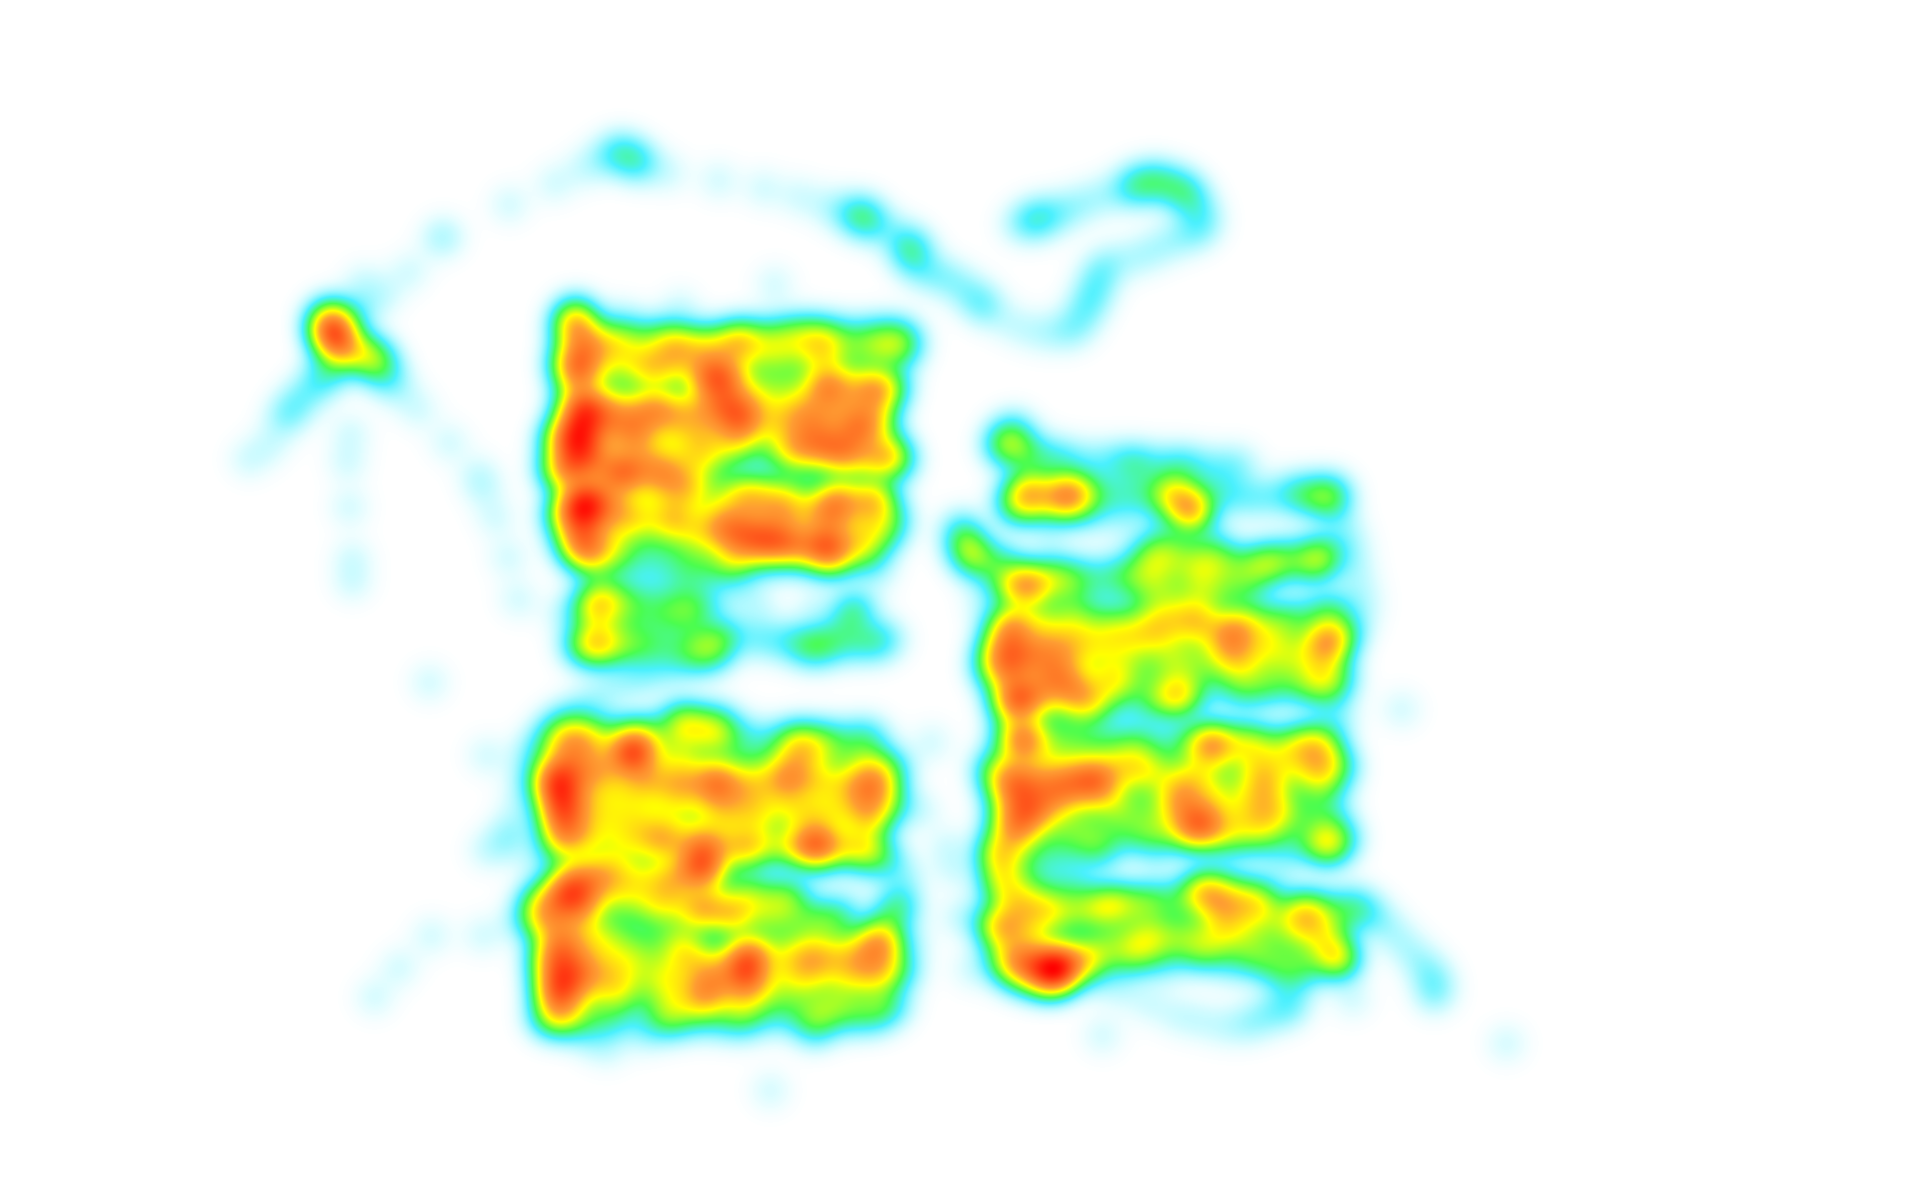
\includegraphics[width=\textwidth]{Images/Heatmaps/firstHeatmapTest.png}
    \caption{Basic test heatmap generated by me from reading one page of a paper.}
    \label{fig:res_FirstHeatMapTest}
\end{figure}

\subsection{Binary classification dataset}

Show some plot that represents the quality of labels

\subsubsection{Human error bias}

As was briefly mentioned in section \ref{sec:meth_DataLabellingEnvironments}, a bias was expected to be introduced in the dataset by human error when the user is prompted to label his own actions by mouse clicks. In figure \ref{fig:res_HumanErrorBias}, we attempt to visualise this bias by using the dispertion feature, described in further detail in section \ref{sec:meth_FeatureGeneration}. As we can see, there is very poor correlation between the peaks of xy-dispertion and each sample's labelled event. This fact reveals the major value of the post-labelling step, employed in dataset represented above. It seems that labelled saccades are lagging the dispertion peaks by a few samples, likely because the user releases the labelling button as he is moving his gaze, and simple human reaction time leads to the observed bias. Additionally, we can see that the sample period of saccade-labelled samples have little correlation with the number of samples with high values of xy-dispersion, nor the length of the saccade. This bias is likely caused by the fact that the user has no way of distinguishing the micro-differences of a 15ms saccade from a 100ms saccade, and consequently label all saccades with the same interval of button release. 

\begin{figure}[h]
    \centering
    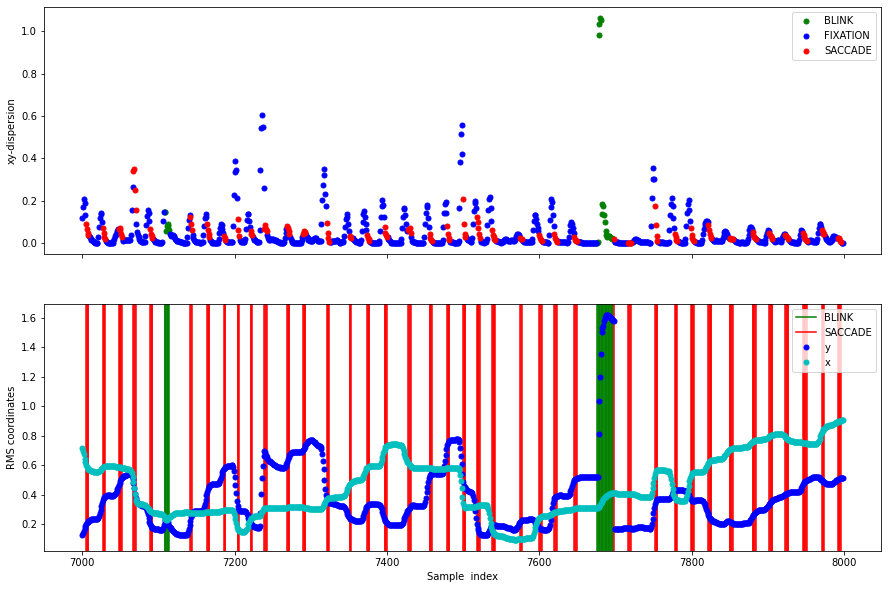
\includegraphics[width=\textwidth]{Images/Dataset/DQ_V1.png}
    \caption{Data quality from manual user labelling in static environment. The top plot show xy-dispersion and the bottom plot show x-y on-screen coordinates. Both plots are taken form a random subset of 1000 samples in the dataset. Red vertical lines and dots indicate samples where a saccade is labelled, and green vertical lines and dots indicate samples where a blink is labelled. Blue dots are samples labelled as a fixation.}
    \label{fig:res_HumanErrorBias}
\end{figure}


\subsection{Multi-class classification dataset}

Show some plot that represents the quality of labels

\subsection{Feature correlations}